% This file contains TikZ diagrams for the research paper
% To be included in the main LaTeX file or compiled separately

\documentclass[tikz,border=10pt]{standalone}
\usepackage{tikz}
\usetikzlibrary{shapes,arrows,positioning,calc}
\usepackage{amsmath}

\begin{document}

% Model Architecture Diagram
\begin{tikzpicture}[node distance=2.5cm, auto, scale=0.8, transform shape]
    % Define styles
    \tikzstyle{block} = [rectangle, draw, fill=blue!20, text width=8em, text centered, minimum height=4em, rounded corners]
    \tikzstyle{inputblock} = [rectangle, draw, fill=green!20, text width=6em, text centered, minimum height=3em]
    \tikzstyle{outputblock} = [rectangle, draw, fill=red!20, text width=6em, text centered, minimum height=3em]
    \tikzstyle{arrow} = [draw, -latex', thick]
    \tikzstyle{smallblock} = [rectangle, draw, fill=yellow!20, text width=5em, text centered, minimum height=2.5em, font=\small]
    \tikzstyle{formulablock} = [rectangle, draw, fill=orange!20, text width=7em, text centered, minimum height=3em]
    
    % Input Layer
    \node[inputblock] (features) {Input\\Features};
    
    % Feature Categories
    \node[smallblock, below left=1.5cm and 0.5cm of features] (context) {Contextual\\Features\\(93)};
    \node[smallblock, below right=1.5cm and 0.5cm of features] (physics) {Physics\\Features\\(36)};
    
    % Formula Calculation
    \node[formulablock, below=2cm of features] (formula) {Formula\\Feature\\Calculation};
    
    % XGBoost Model
    \node[block, below=2cm of formula] (xgboost) {XGBoost\\Multi-Output\\Regressor};
    
    % Output Layer
    \node[outputblock, below=2cm of xgboost] (output) {Predictions};
    
    % Output Details
    \node[smallblock, below left=0.5cm and 0.5cm of output] (c_mat) {Carbon\\Material};
    \node[smallblock, below=0.5cm of output] (c_trans) {Carbon\\Transport};
    \node[smallblock, below=0.5cm and right=0.5cm of output] (c_total) {Carbon\\Total};
    \node[smallblock, below right=0.5cm and 0.5cm of output] (w_total) {Water\\Total};
    
    % Arrows
    \draw[arrow] (features) -- (context);
    \draw[arrow] (features) -- (physics);
    \draw[arrow] (context) -- (formula);
    \draw[arrow] (physics) -- (formula);
    \draw[arrow] (formula) -- (xgboost);
    \draw[arrow] (xgboost) -- (output);
    \draw[arrow] (output) -- (c_mat);
    \draw[arrow] (output) -- (c_trans);
    \draw[arrow] (output) -- (c_total);
    \draw[arrow] (output) -- (w_total);
    
    % Labels
    \node[above=0.2cm of features] {Input Layer};
    \node[above=0.2cm of formula] {Feature Engineering};
    \node[above=0.2cm of xgboost] {Model Core};
    \node[above=0.2cm of output] {Output Layer};
    
    % Feature details
    \node[below=0.3cm of context, font=\tiny, align=center] {Gender\\Parent Cat.\\Category};
    \node[below=0.3cm of physics, font=\tiny, align=center] {Weight\\Distance\\Materials};
    
    % Title
    \node[above=0.5cm of features] {\Large \textbf{HydroCarbon Model Architecture}};
\end{tikzpicture}

% Training Process Diagram
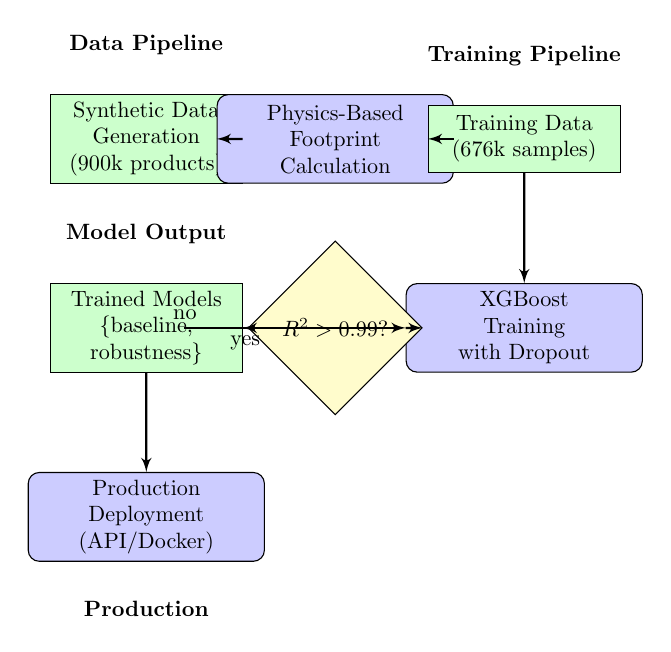
\begin{tikzpicture}[node distance=3cm, auto, scale=0.8, transform shape]
    \tikzstyle{process} = [rectangle, draw, fill=blue!20, text width=10em, text centered, minimum height=4em, rounded corners]
    \tikzstyle{data} = [rectangle, draw, fill=green!20, text width=8em, text centered, minimum height=3em]
    \tikzstyle{arrow} = [draw, -latex', thick]
    \tikzstyle{decision} = [diamond, draw, fill=yellow!20, text width=7em, text badly centered, inner sep=0pt]
    
    % Data Generation
    \node[data] (synthetic) {Synthetic Data\\Generation\\(900k products)};
    
    % Physics Calculation
    \node[process, right of=synthetic] (physics) {Physics-Based\\Footprint\\Calculation};
    
    % Training Data
    \node[data, right of=physics] (training) {Training Data\\(676k samples)};
    
    % XGBoost Training
    \node[process, below of=training] (train) {XGBoost\\Training\\with Dropout};
    
    % Validation
    \node[decision, left of=train] (val) {$R^2 > 0.99$?};
    
    % Models
    \node[data, left of=val] (models) {Trained Models\\\{baseline, robustness\}};
    
    % Deployment
    \node[process, below of=models] (deploy) {Production\\Deployment\\(API/Docker)};
    
    % Arrows
    \draw[arrow] (synthetic) -- (physics);
    \draw[arrow] (physics) -- (training);
    \draw[arrow] (training) -- (train);
    \draw[arrow] (train) -- (val);
    \draw[arrow] (val) -- node {yes} (models);
    \draw[arrow] (val.west) -- ++(-1,0) node[above] {no} |- (train.west);
    \draw[arrow] (models) -- (deploy);
    
    % Labels
    \node[above=0.5cm of synthetic] {\textbf{Data Pipeline}};
    \node[above=0.5cm of training] {\textbf{Training Pipeline}};
    \node[above=0.5cm of models] {\textbf{Model Output}};
    \node[below=0.5cm of deploy] {\textbf{Production}};
\end{tikzpicture}

% Performance Comparison Chart (Bar Chart)
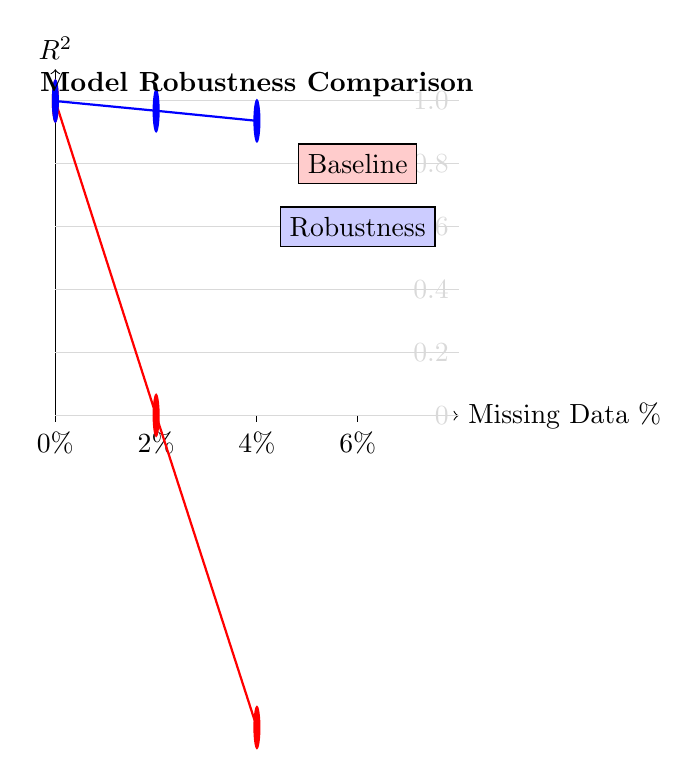
\begin{tikzpicture}[scale=0.8]
    \begin{scope}[xscale=0.8, yscale=5]
        % R² values
        \draw[->] (0,0) -- (8,0) node[right] {Missing Data \%};
        \draw[->] (0,0) -- (0,1.1) node[above] {$R^2$};
        
        % Grid lines
        \foreach \y in {0,0.2,0.4,0.6,0.8,1.0}
            \draw[gray!30] (0,\y) -- (8,\y) node[left] {\y};
        
        % X-axis labels
        \foreach \x in {0,2,4,6}
            \draw (\x,0) -- (\x,-0.02) node[below] {\x\%};
        
        % Baseline model points
        \fill[red] (0,0.999) circle (2pt);
        \fill[red] (2,0.001) circle (2pt);
        \fill[red] (4,-0.99) circle (2pt);
        \draw[red, thick] (0,0.999) -- (2,0.001) -- (4,-0.99);
        
        % Robustness model points
        \fill[blue] (0,0.999) circle (2pt);
        \fill[blue] (2,0.968) circle (2pt);
        \fill[blue] (4,0.936) circle (2pt);
        \draw[blue, thick] (0,0.999) -- (2,0.968) -- (4,0.936);
        
        % Legend
        \node[draw, fill=red!20, minimum width=1cm, minimum height=0.5cm] at (6,0.8) {Baseline};
        \node[draw, fill=blue!20, minimum width=1cm, minimum height=0.5cm] at (6,0.6) {Robustness};
        
        % Title
        \node at (4,1.05) {\textbf{Model Robustness Comparison}};
    \end{scope}
\end{tikzpicture}

% Modal Split Example
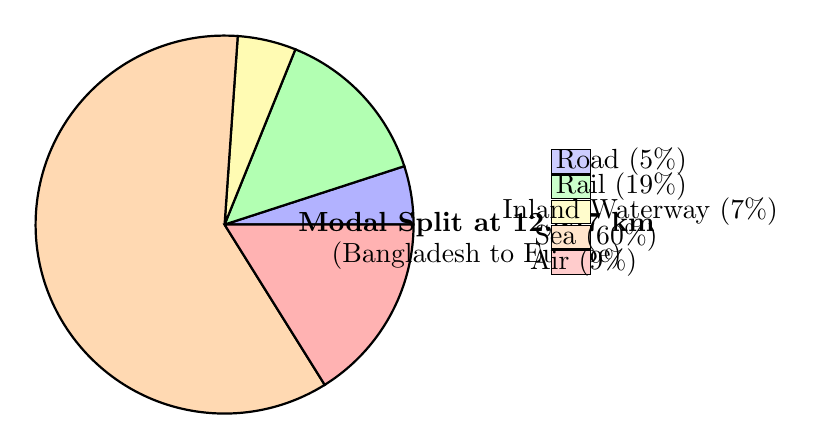
\begin{tikzpicture}[scale=0.8]
    \tikzstyle{slice} = [draw, thick]
    
    % Pie chart for D = 12,847 km
    \draw[slice, fill=blue!30] (0,0) -- (3,0) arc (0:18:3) -- cycle;
    \draw[slice, fill=green!30] (0,0) -- ({3*cos(18)}, {3*sin(18)}) arc (18:68:3) -- cycle;
    \draw[slice, fill=yellow!30] (0,0) -- ({3*cos(68)}, {3*sin(68)}) arc (68:86:3) -- cycle;
    \draw[slice, fill=orange!30] (0,0) -- ({3*cos(86)}, {3*sin(86)}) arc (86:302:3) -- cycle;
    \draw[slice, fill=red!30] (0,0) -- ({3*cos(302)}, {3*sin(302)}) arc (302:360:3) -- cycle;
    
    % Labels
    \node at (4,0) {\textbf{Modal Split at 12,847 km}};
    \node at (4,-0.5) {(Bangladesh to Europe)};
    
    % Legend
    \node[draw, fill=blue!20, minimum width=0.5cm, minimum height=0.3cm] at (5.5,1) {};
    \node at (6.3,1) {Road (5\%)};
    
    \node[draw, fill=green!20, minimum width=0.5cm, minimum height=0.3cm] at (5.5,0.6) {};
    \node at (6.3,0.6) {Rail (19\%)};
    
    \node[draw, fill=yellow!20, minimum width=0.5cm, minimum height=0.3cm] at (5.5,0.2) {};
    \node at (6.6,0.2) {Inland Waterway (7\%)};
    
    \node[draw, fill=orange!20, minimum width=0.5cm, minimum height=0.3cm] at (5.5,-0.2) {};
    \node at (5.9,-0.2) {Sea (60\%)};
    
    \node[draw, fill=red!20, minimum width=0.5cm, minimum height=0.3cm] at (5.5,-0.6) {};
    \node at (5.7,-0.6) {Air (9\%)};
\end{tikzpicture}

\end{document}
